% Options for packages loaded elsewhere
\PassOptionsToPackage{unicode}{hyperref}
\PassOptionsToPackage{hyphens}{url}
\PassOptionsToPackage{dvipsnames,svgnames,x11names}{xcolor}
%
\documentclass[
]{agujournal2019}

\usepackage{amsmath,amssymb}
\usepackage{iftex}
\ifPDFTeX
  \usepackage[T1]{fontenc}
  \usepackage[utf8]{inputenc}
  \usepackage{textcomp} % provide euro and other symbols
\else % if luatex or xetex
  \usepackage{unicode-math}
  \defaultfontfeatures{Scale=MatchLowercase}
  \defaultfontfeatures[\rmfamily]{Ligatures=TeX,Scale=1}
\fi
\usepackage{lmodern}
\ifPDFTeX\else  
    % xetex/luatex font selection
\fi
% Use upquote if available, for straight quotes in verbatim environments
\IfFileExists{upquote.sty}{\usepackage{upquote}}{}
\IfFileExists{microtype.sty}{% use microtype if available
  \usepackage[]{microtype}
  \UseMicrotypeSet[protrusion]{basicmath} % disable protrusion for tt fonts
}{}
\makeatletter
\@ifundefined{KOMAClassName}{% if non-KOMA class
  \IfFileExists{parskip.sty}{%
    \usepackage{parskip}
  }{% else
    \setlength{\parindent}{0pt}
    \setlength{\parskip}{6pt plus 2pt minus 1pt}}
}{% if KOMA class
  \KOMAoptions{parskip=half}}
\makeatother
\usepackage{xcolor}
\setlength{\emergencystretch}{3em} % prevent overfull lines
\setcounter{secnumdepth}{5}
% Make \paragraph and \subparagraph free-standing
\makeatletter
\ifx\paragraph\undefined\else
  \let\oldparagraph\paragraph
  \renewcommand{\paragraph}{
    \@ifstar
      \xxxParagraphStar
      \xxxParagraphNoStar
  }
  \newcommand{\xxxParagraphStar}[1]{\oldparagraph*{#1}\mbox{}}
  \newcommand{\xxxParagraphNoStar}[1]{\oldparagraph{#1}\mbox{}}
\fi
\ifx\subparagraph\undefined\else
  \let\oldsubparagraph\subparagraph
  \renewcommand{\subparagraph}{
    \@ifstar
      \xxxSubParagraphStar
      \xxxSubParagraphNoStar
  }
  \newcommand{\xxxSubParagraphStar}[1]{\oldsubparagraph*{#1}\mbox{}}
  \newcommand{\xxxSubParagraphNoStar}[1]{\oldsubparagraph{#1}\mbox{}}
\fi
\makeatother


\providecommand{\tightlist}{%
  \setlength{\itemsep}{0pt}\setlength{\parskip}{0pt}}\usepackage{longtable,booktabs,array}
\usepackage{calc} % for calculating minipage widths
% Correct order of tables after \paragraph or \subparagraph
\usepackage{etoolbox}
\makeatletter
\patchcmd\longtable{\par}{\if@noskipsec\mbox{}\fi\par}{}{}
\makeatother
% Allow footnotes in longtable head/foot
\IfFileExists{footnotehyper.sty}{\usepackage{footnotehyper}}{\usepackage{footnote}}
\makesavenoteenv{longtable}
\usepackage{graphicx}
\makeatletter
\newsavebox\pandoc@box
\newcommand*\pandocbounded[1]{% scales image to fit in text height/width
  \sbox\pandoc@box{#1}%
  \Gscale@div\@tempa{\textheight}{\dimexpr\ht\pandoc@box+\dp\pandoc@box\relax}%
  \Gscale@div\@tempb{\linewidth}{\wd\pandoc@box}%
  \ifdim\@tempb\p@<\@tempa\p@\let\@tempa\@tempb\fi% select the smaller of both
  \ifdim\@tempa\p@<\p@\scalebox{\@tempa}{\usebox\pandoc@box}%
  \else\usebox{\pandoc@box}%
  \fi%
}
% Set default figure placement to htbp
\def\fps@figure{htbp}
\makeatother
% definitions for citeproc citations
\NewDocumentCommand\citeproctext{}{}
\NewDocumentCommand\citeproc{mm}{%
  \begingroup\def\citeproctext{#2}\cite{#1}\endgroup}
\makeatletter
 % allow citations to break across lines
 \let\@cite@ofmt\@firstofone
 % avoid brackets around text for \cite:
 \def\@biblabel#1{}
 \def\@cite#1#2{{#1\if@tempswa , #2\fi}}
\makeatother
\newlength{\cslhangindent}
\setlength{\cslhangindent}{1.5em}
\newlength{\csllabelwidth}
\setlength{\csllabelwidth}{3em}
\newenvironment{CSLReferences}[2] % #1 hanging-indent, #2 entry-spacing
 {\begin{list}{}{%
  \setlength{\itemindent}{0pt}
  \setlength{\leftmargin}{0pt}
  \setlength{\parsep}{0pt}
  % turn on hanging indent if param 1 is 1
  \ifodd #1
   \setlength{\leftmargin}{\cslhangindent}
   \setlength{\itemindent}{-1\cslhangindent}
  \fi
  % set entry spacing
  \setlength{\itemsep}{#2\baselineskip}}}
 {\end{list}}
\usepackage{calc}
\newcommand{\CSLBlock}[1]{\hfill\break\parbox[t]{\linewidth}{\strut\ignorespaces#1\strut}}
\newcommand{\CSLLeftMargin}[1]{\parbox[t]{\csllabelwidth}{\strut#1\strut}}
\newcommand{\CSLRightInline}[1]{\parbox[t]{\linewidth - \csllabelwidth}{\strut#1\strut}}
\newcommand{\CSLIndent}[1]{\hspace{\cslhangindent}#1}

\usepackage{url} %this package should fix any errors with URLs in refs.
\usepackage{lineno}
\usepackage[inline]{trackchanges} %for better track changes. finalnew option will compile document with changes incorporated.
\usepackage{soul}
\linenumbers
\makeatletter
\@ifpackageloaded{caption}{}{\usepackage{caption}}
\AtBeginDocument{%
\ifdefined\contentsname
  \renewcommand*\contentsname{Table of contents}
\else
  \newcommand\contentsname{Table of contents}
\fi
\ifdefined\listfigurename
  \renewcommand*\listfigurename{List of Figures}
\else
  \newcommand\listfigurename{List of Figures}
\fi
\ifdefined\listtablename
  \renewcommand*\listtablename{List of Tables}
\else
  \newcommand\listtablename{List of Tables}
\fi
\ifdefined\figurename
  \renewcommand*\figurename{Figure}
\else
  \newcommand\figurename{Figure}
\fi
\ifdefined\tablename
  \renewcommand*\tablename{Table}
\else
  \newcommand\tablename{Table}
\fi
}
\@ifpackageloaded{float}{}{\usepackage{float}}
\floatstyle{ruled}
\@ifundefined{c@chapter}{\newfloat{codelisting}{h}{lop}}{\newfloat{codelisting}{h}{lop}[chapter]}
\floatname{codelisting}{Listing}
\newcommand*\listoflistings{\listof{codelisting}{List of Listings}}
\makeatother
\makeatletter
\makeatother
\makeatletter
\@ifpackageloaded{caption}{}{\usepackage{caption}}
\@ifpackageloaded{subcaption}{}{\usepackage{subcaption}}
\makeatother

\usepackage{bookmark}

\IfFileExists{xurl.sty}{\usepackage{xurl}}{} % add URL line breaks if available
\urlstyle{same} % disable monospaced font for URLs
\hypersetup{
  pdftitle={Shifting paradigms in Ocean Color: Bayesian Inference for Uncertainty-Aware Chlorophyll Estimation},
  pdfauthor={Erdem M. Karaköylü; Susanne E. Craig},
  pdfkeywords={Bayesian modeling, Ocean Color},
  colorlinks=true,
  linkcolor={blue},
  filecolor={Maroon},
  citecolor={Blue},
  urlcolor={Blue},
  pdfcreator={LaTeX via pandoc}}


\journalname{Remote Sensing of Environment}

\draftfalse

\begin{document}
\title{Shifting paradigms in Ocean Color: Bayesian Inference for
Uncertainty-Aware Chlorophyll Estimation}

\authors{Erdem M. Karaköylü\affil{1}, Susanne E. Craig\affil{2}}
\affiliation{1}{Independent Researcher, }\affiliation{2}{NASA/UMBC, }
\correspondingauthor{Erdem M. Karaköylü}{erdemk@protonmail.com}


\begin{abstract}
Placeholder
\end{abstract}

\section*{Plain Language Summary}
Placeholder




\section{Introduction}\label{introduction}

Satellite ocean color remote sensing has long served as a cornerstone of
marine ecosystem monitoring, offering global and synoptic coverage of
surface ocean properties. Among these, chlorophyll-a (\(Chl_a\))
concentration remains a central metric, widely used as a proxy for
phytoplankton biomass, primary production, and water quality. The
retrieval of \(Chl_a\) from ocean color data has evolved over decades,
resulting in a diverse lineage of empirical and semi-empirical
algorithms. The following section summarizes this historical
development, which sets the stage for a critical examination of the
statistical foundations underlying current approaches.

\subsection{Historical Context of Chlorophyll
Algorithms}\label{historical-context-of-chlorophyll-algorithms}

Satellite ocean color observations have long been fundamental for
monitoring marine ecosystems, as they enable global estimation of
chlorophyll‑a (\(Chl_a\)) --- a key indicator of phytoplankton biomass
and ocean productivity. Early empirical algorithms, notably developed by
O'Reilly et al. (John E. O'Reilly et al., 1998; John E. O'Reilly et al.,
2000), established the \(OCx\) family (where \(x\) denotes the number of
bands used) of polynomial regression models. These models relate
blue-to-green reflectance ratios (after log‑transformation) to in situ
\(Chl_a\), employing either straight band ratios (BR) or maximum band
ratios (MBR)---the latter selecting the highest available blue-to-green
ratio for any given observation as input to a high‑order polynomial.
These formulations have served as the operational foundation for
chlorophyll‑a products across a broad range of satellite ocean color
sensors---from the pioneering Coastal Zone Color Scanner (CZCS) through
SeaWiFS, MODIS, and MERIS to more recent missions---offering a
straightforward and robust approach for Case‑1 waters. However, their
performance is more limited in optically complex Case‑2 waters and
remains sensitive to atmospheric correction errors.

Subsequent refinements were introduced to address these deficiencies.
For example, Hu et al. (Hu et al., 2012) proposed a Color Index (CI)
formulation that employs a band‑difference approach to reduce
sensitivity to residual atmospheric errors and instrument noise, with
further improvements enhancing inter‑sensor agreement (Hu et al., 2019).
The increasing availability of calibration data (e.g.,
(\textbf{Valente2015?})) and ongoing algorithmic improvements have led
to the development of additional variants of the \(OCx\)
algorithms---specifically, the OC5 and OC6 formulations. O'Reilly and
Werdell (John E. O'Reilly \& Werdell, 2019) maintain that OC5 extends
the spectral basis by incorporating the 412\,nm band, thereby exploiting
its strong signal in clear, oligotrophic waters, while OC6 replaces the
traditional denominator with the mean of the 555 and 670\,nm
reflectances, with the aim of improving the dynamic range at low
chlorophyll concentrations. In total, (John E. O'Reilly \& Werdell,
2019) propose 65 versions of BR/MBR \(OCx\) type algorithms for 25
sensors---on average, two or more variants per sensor. With this
arsenal, it is hoped, researchers are better equipped to address the
wide array of bio‑optical environments encountered in global ocean color
applications.

\subsection{Limitations of Existing
Approaches}\label{limitations-of-existing-approaches}

Regrettably, the development of traditional ocean color algorithms is
grounded in a fundamental statistical error---one that pervades much of
observational science: the conflation of sampling probability with
inferential probability (Jaynes \& Bretthorst, 2003;
\textbf{DeScheemaekere2011?}).

Consider a dataset \(D\) composed of input--output pairs---e.g., remote
sensing reflectance (Rrs) and chlorophyll-a concentration
(\(Chl_a\))---and a model \(M\), such as OCx, posited to represent the
relationship between them. The sampling probability \(p(D \mid M)\)
denotes the probability of observing data \(D\) under the assumption
that model \(M\) is true. In standard model fitting, this likelihood is
maximized by adjusting the parameters of \(M\) to best explain the
observed data.

This approach tacitly assumes that the model which best fits the data
also most accurately represents the underlying generative process. This
constitutes an epistemic fallacy---treating \(p(D \mid M)\) as if it
were \(p(M \mid D)\)---a direct violation of Bayes' theorem and the
rules governing conditional probability.

Although in well-behaved, data-rich cases---where the likelihood is
regular, the signal strong, and the model adequately constrained---the
maxima of \(p(D \mid M)\) and \(p(M \mid D)\) may coincide, this remains
the exception---not the rule.

This mistake lies at the heart of what Clayton (Clayton, 2022) terms the
Bernoulli Fallacy: the widespread misinterpretation of likelihood as
inference, or of data-fit as belief. As Clayton argues, this logical
misstep has far-reaching consequences, with implications that extend
beyond science to domains such as medicine, law, and public policy.

In scientific modeling, this fallacy contributes to poor generalization,
drives the use of ad hoc or retrospective uncertainty quantification,
and underlies many published results that later prove difficult to
replicate (Baker, 2016; Cobey et al., 2024). These limitations are not
restricted to classical hypothesis testing; they persist in the training
and deployment of modern machine learning models as well.

In regression and classification, maximizing likelihood is often treated
as sufficient for inference---despite yielding only a single point
estimate and ignoring both parameter uncertainty and the plausibility of
alternative models.

This epistemic shortcut has been directly critiqued in the machine
learning literature. Gal (Gal, 2016) and Ghahramani
(\textbf{gahramani2015probabilistic?}) point out that most ML models
discard uncertainty altogether, treating the outcome of an optimization
as if it were an inference. The result is overconfident predictions and
brittle generalization---concerns that echo Clayton's critique.

Bishop (Bishop, 2006) similarly distinguishes between the utility of
predictive models and the inferential scaffolding required to quantify
uncertainty, reinforcing the notion that likelihood alone is
insufficient---and that the Bernoulli Fallacy permeates much of applied
machine learning.

\subsection{Overcoming limitations}\label{overcoming-limitations}

Several recent efforts have attempted to address the limitations of
classical retrieval models. For instance, (Seegers et al., 2018)
proposed alternative evaluation metrics to move beyond restrictive
frequentist assumptions. Others have incorporated Bayesian elements into
the modeling pipeline: (Frouin \& Pelletier, 2013) applied Bayesian
inversion for atmospheric correction, (\textbf{shi2015?}) used
probabilistic fusion for multi-sensor data, and (Craig \& Karaköylü,
2019) employed Hamiltonian Monte Carlo to train Bayesian neural networks
(BNNs) for retrieving inherent optical properties (IOPs) from
top-of-atmosphere radiance. Similarly, (\textbf{werther2022?})
introduced Monte Carlo dropout as an approximate BNN strategy, while
(Erickson et al., 2023) recast the Generalized Inherent Optical Property
(GIOP) framework using conjugate Bayesian linear models. Most recently,
(\textbf{hammout2024?}) developed a BNN surrogate using stochastic
variational inference for chlorophyll-a prediction from Rrs.

While these studies mark important progress, they often adopt only
isolated components of what has come to be known as the Bayesian
workflow (\textbf{bgelman2019?}). Key aspects---such as principled prior
specification, posterior predictive checking, and formal model
comparison---remain largely absent. As a result, uncertainty is
frequently approximated rather than inferred, and model structure is
rarely treated as a variable to be interrogated.

This paper builds on prior work and extends it by applying a fully
Bayesian modeling framework for chlorophyll-a prediction from sea
surface reflectance (Rrs), with explicit treatment of uncertainty, model
complexity, and measurement error.

\section{Materials and Methods}\label{materials-and-methods}

This section outlines the dataset, model structures, inference methods,
and model evaluation criteria used in this study. I focus on a fully
Bayesian approach to modeling chlorophyll-a from satellite remote
sensing reflectance (Rrs), emphasizing transparency, uncertainty
quantification, and principled model comparison. Four models are
presented in the main text, while all six model formulations and results
are included in the Supplement.

\subsection{Data Description and Preparation
Overview}\label{data-description-and-preparation-overview}

For pedagogical reasons, I used the well known NOMAD (Werdell \& Bailey,
2005) dataset, which includes quality-controlled in situ measurements of
chlorophyll-a matched with coincident satellite Rrs data. These
measurements span a range of oceanographic conditions, enabling the
development of models that are expected to generalize across water
types. The data were loaded using the Python Pandas library (team,
2020), which was used for all subsequent cleaning, preprocessing, and
transformation operations.

\emph{Raw Data} - Sea-surface reflectances (Rrs) in the 6 visible
SeaWiFS bands (411, 443, 489, 510, 550, 670nm) constitue the bulk of the
data. Chlorophyll concentrations, measured via fluorescence or HPLC or
both, consituted the target variables. Any row containing an invalid
data point (null, zero, or negative) was removed, as proper
missing/invalid data imputation is a subject onto itself and beyond the
scope of this paper.

\emph{Data Preprocessing and Transformation} - Chlorophyll measurements
from the two different methods were combined into a single data. An
auxiliary column was used to flag the measurement method as `fluo' of
`hplc'. The chlorophyll was then log-transformed to stabilize its
variance. The max band ratio (MBR) was computed as
\(\frac {\max(Rrs411, Rrs443, Rrs489, Rrs)}{Rrs555 + Rrs670}\), similar
to the OC6 model proposed by (John E. O'Reilly \& Werdell, 2019).
Another ancillary column was created to captured the actual Rrs band
used for each set observations. This numerator type as well as the
chlorophyll measurement type are useful to build more hierarchical
partial pooling models that can take advantage of such data groups. A
sample from the fully processed data used in the subsequent models can
be seen in (\textbf{data-table?}).

\phantomsection\label{data-table}
\begin{longtable}[]{@{}
  >{\raggedleft\arraybackslash}p{(\linewidth - 8\tabcolsep) * \real{0.0641}}
  >{\raggedright\arraybackslash}p{(\linewidth - 8\tabcolsep) * \real{0.3077}}
  >{\raggedright\arraybackslash}p{(\linewidth - 8\tabcolsep) * \real{0.1538}}
  >{\raggedright\arraybackslash}p{(\linewidth - 8\tabcolsep) * \real{0.3077}}
  >{\raggedright\arraybackslash}p{(\linewidth - 8\tabcolsep) * \real{0.1667}}@{}}
\toprule\noalign{}
\begin{minipage}[b]{\linewidth}\raggedleft
\end{minipage} & \begin{minipage}[b]{\linewidth}\raggedright
log\_MBR
\end{minipage} & \begin{minipage}[b]{\linewidth}\raggedright
MBR\_flag
\end{minipage} & \begin{minipage}[b]{\linewidth}\raggedright
log\_chl
\end{minipage} & \begin{minipage}[b]{\linewidth}\raggedright
hplc\_flag
\end{minipage} \\
\midrule\noalign{}
\endhead
\bottomrule\noalign{}
\endlastfoot
905 & -0.2545615131431814 & Rrs510 & 0.5837653682849998 & hplc \\
91 & -0.3641327253450254 & Rrs510 & 1.0511525224473812 & fluo \\
528 & -0.0737170739918758 & Rrs510 & 0.14363923527454328 & fluo \\
969 & 0.5813600497877703 & Rrs411 & -0.8272803386505035 & fluo \\
552 & 0.7134341855521412 & Rrs443 & -0.9318141382538383 & hplc \\
\end{longtable}

A random 5-row sample from the Pandas dataframe holding the data used in
subsequent models. \emph{log\_MBR} is the log-transformed Max. Band
Ratio (MBR) of sea surface reflectances, where the numerator is
Max(Rrs411, Rrs443, Rrs489, Rrs510) and the denominator is computed from
the sum of Rrs555 and Rrs670. \emph{MBR\_flag} indicates which of the 4
possible Rrs bands is used in the numerator for that particular row.
\emph{log\_chl} is log transformed in-situ measured chlorophyll \emph{a}
concentration, originally in \(mg\ m^{-3}\). \emph{hplc\_flag} is a
binary variable indicating whether the measurement was obtained via HPLC
or fluorometry. ``-flag'' are used during modeling for grouping data for
hierarchical partial pooling models, explained further below. These
groupings can be seen in Figure~\ref{fig-eda}

\begin{figure}

\begin{minipage}{0.50\linewidth}

\centering{

\pandocbounded{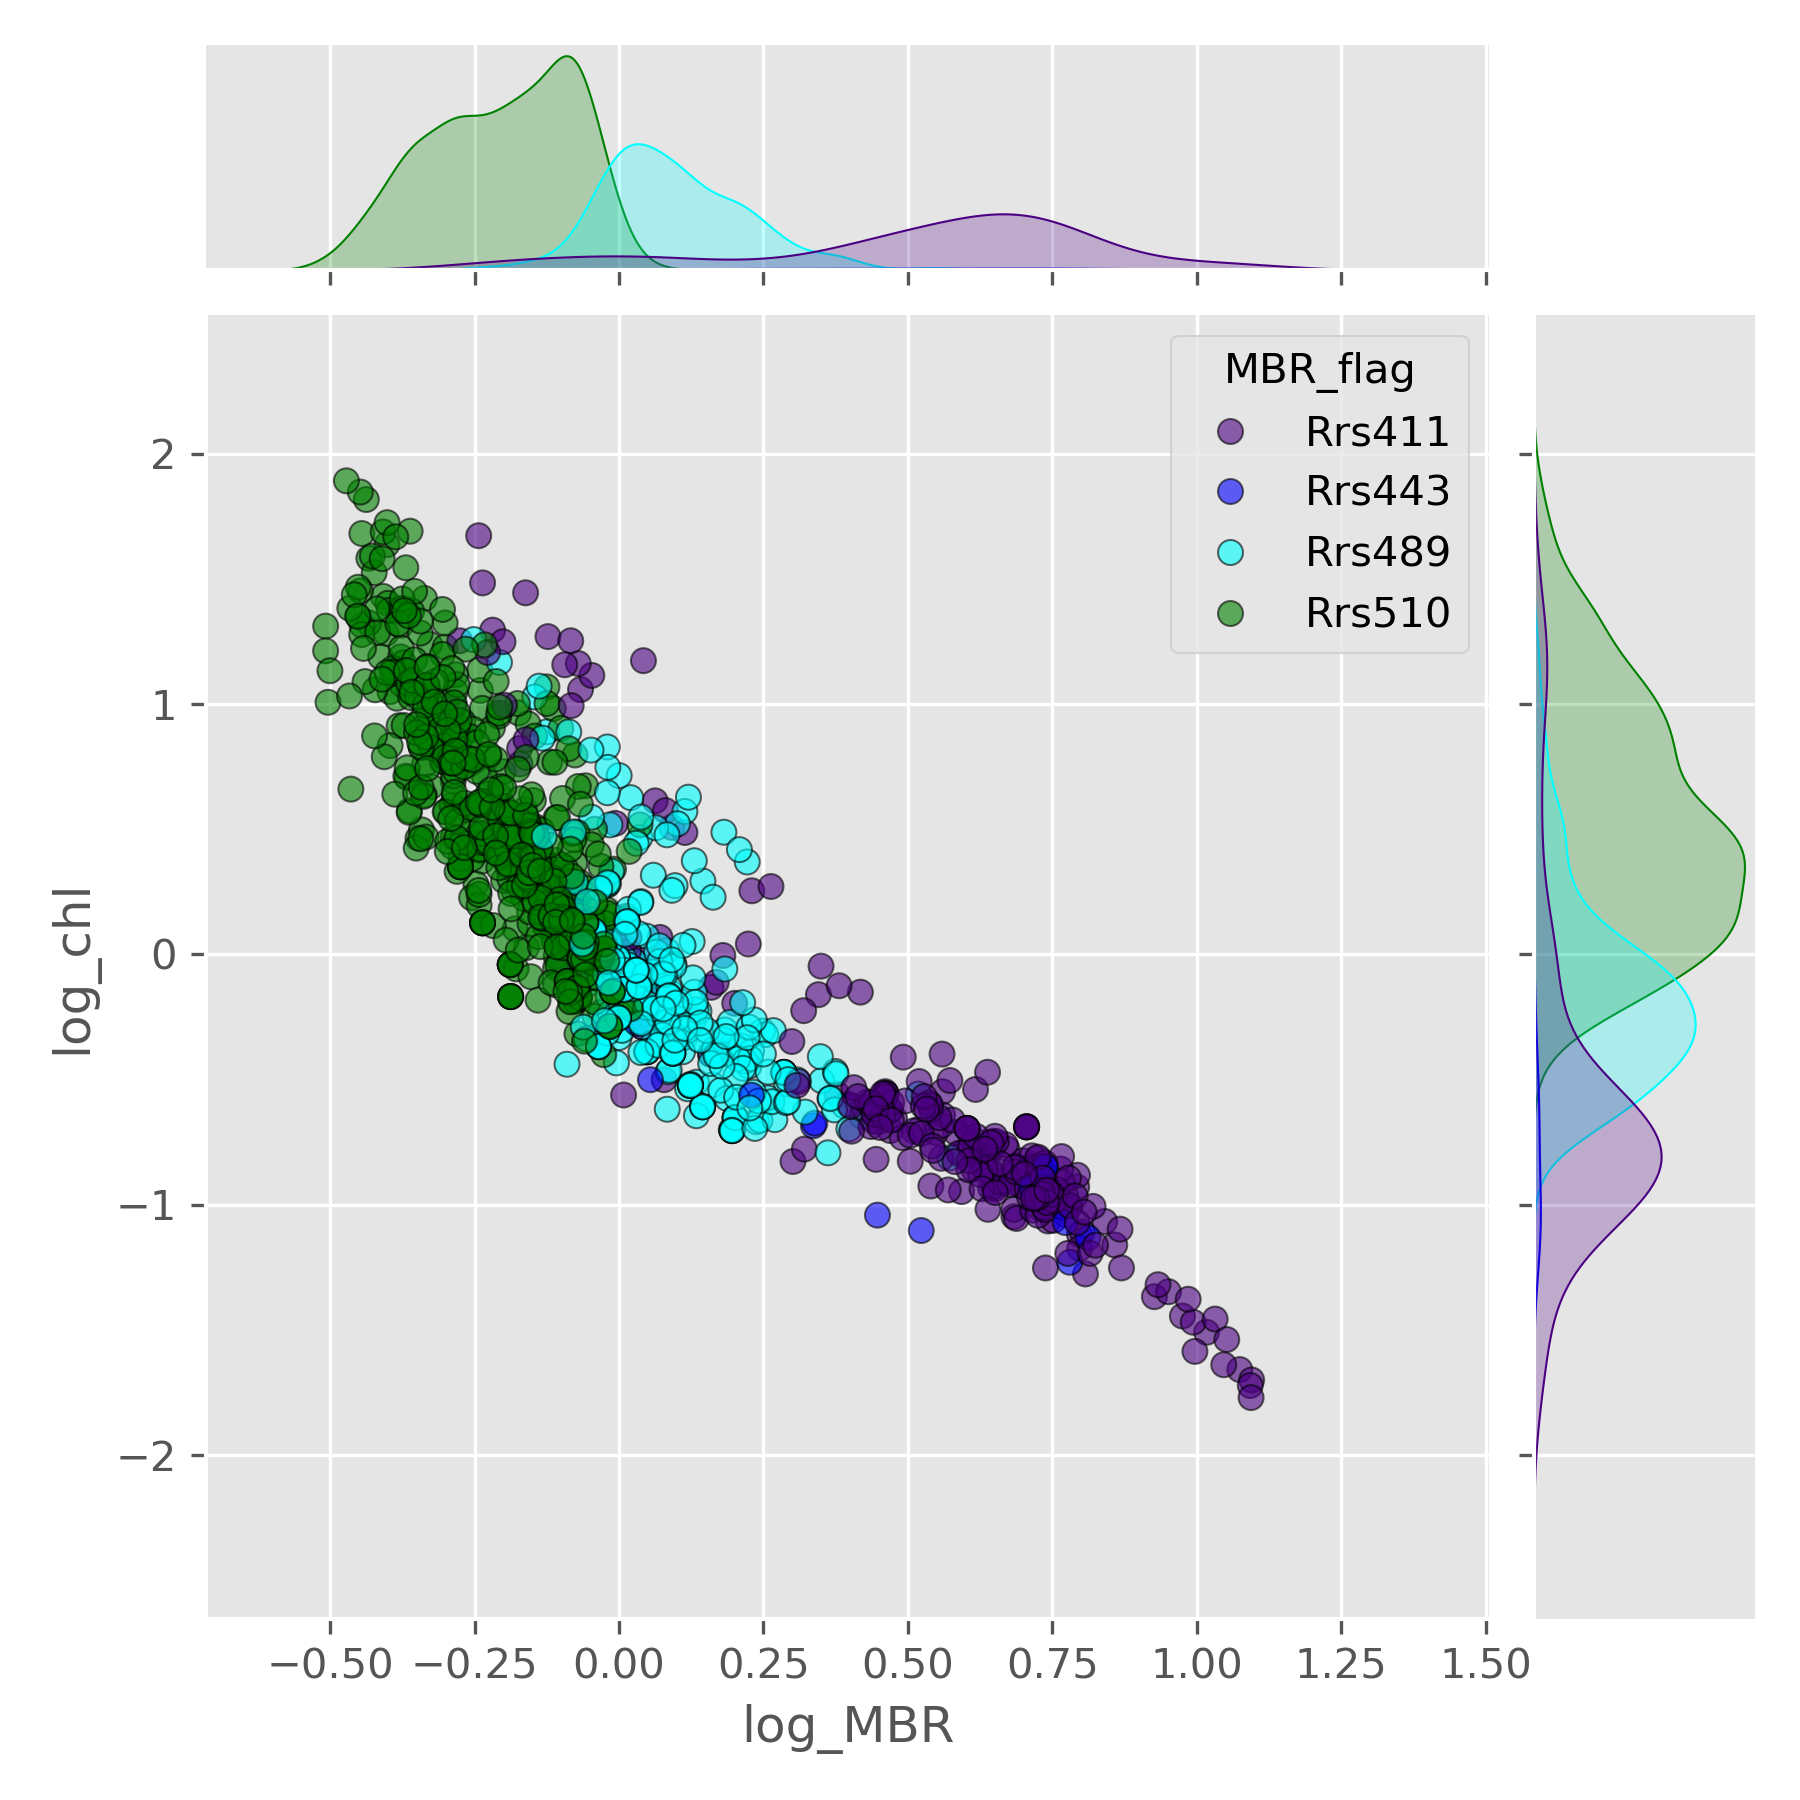
\includegraphics[keepaspectratio]{images/eda_numerator.png}}

}

\subcaption{\label{fig-eda-mbr}}

\end{minipage}%
%
\begin{minipage}{0.50\linewidth}

\centering{

\pandocbounded{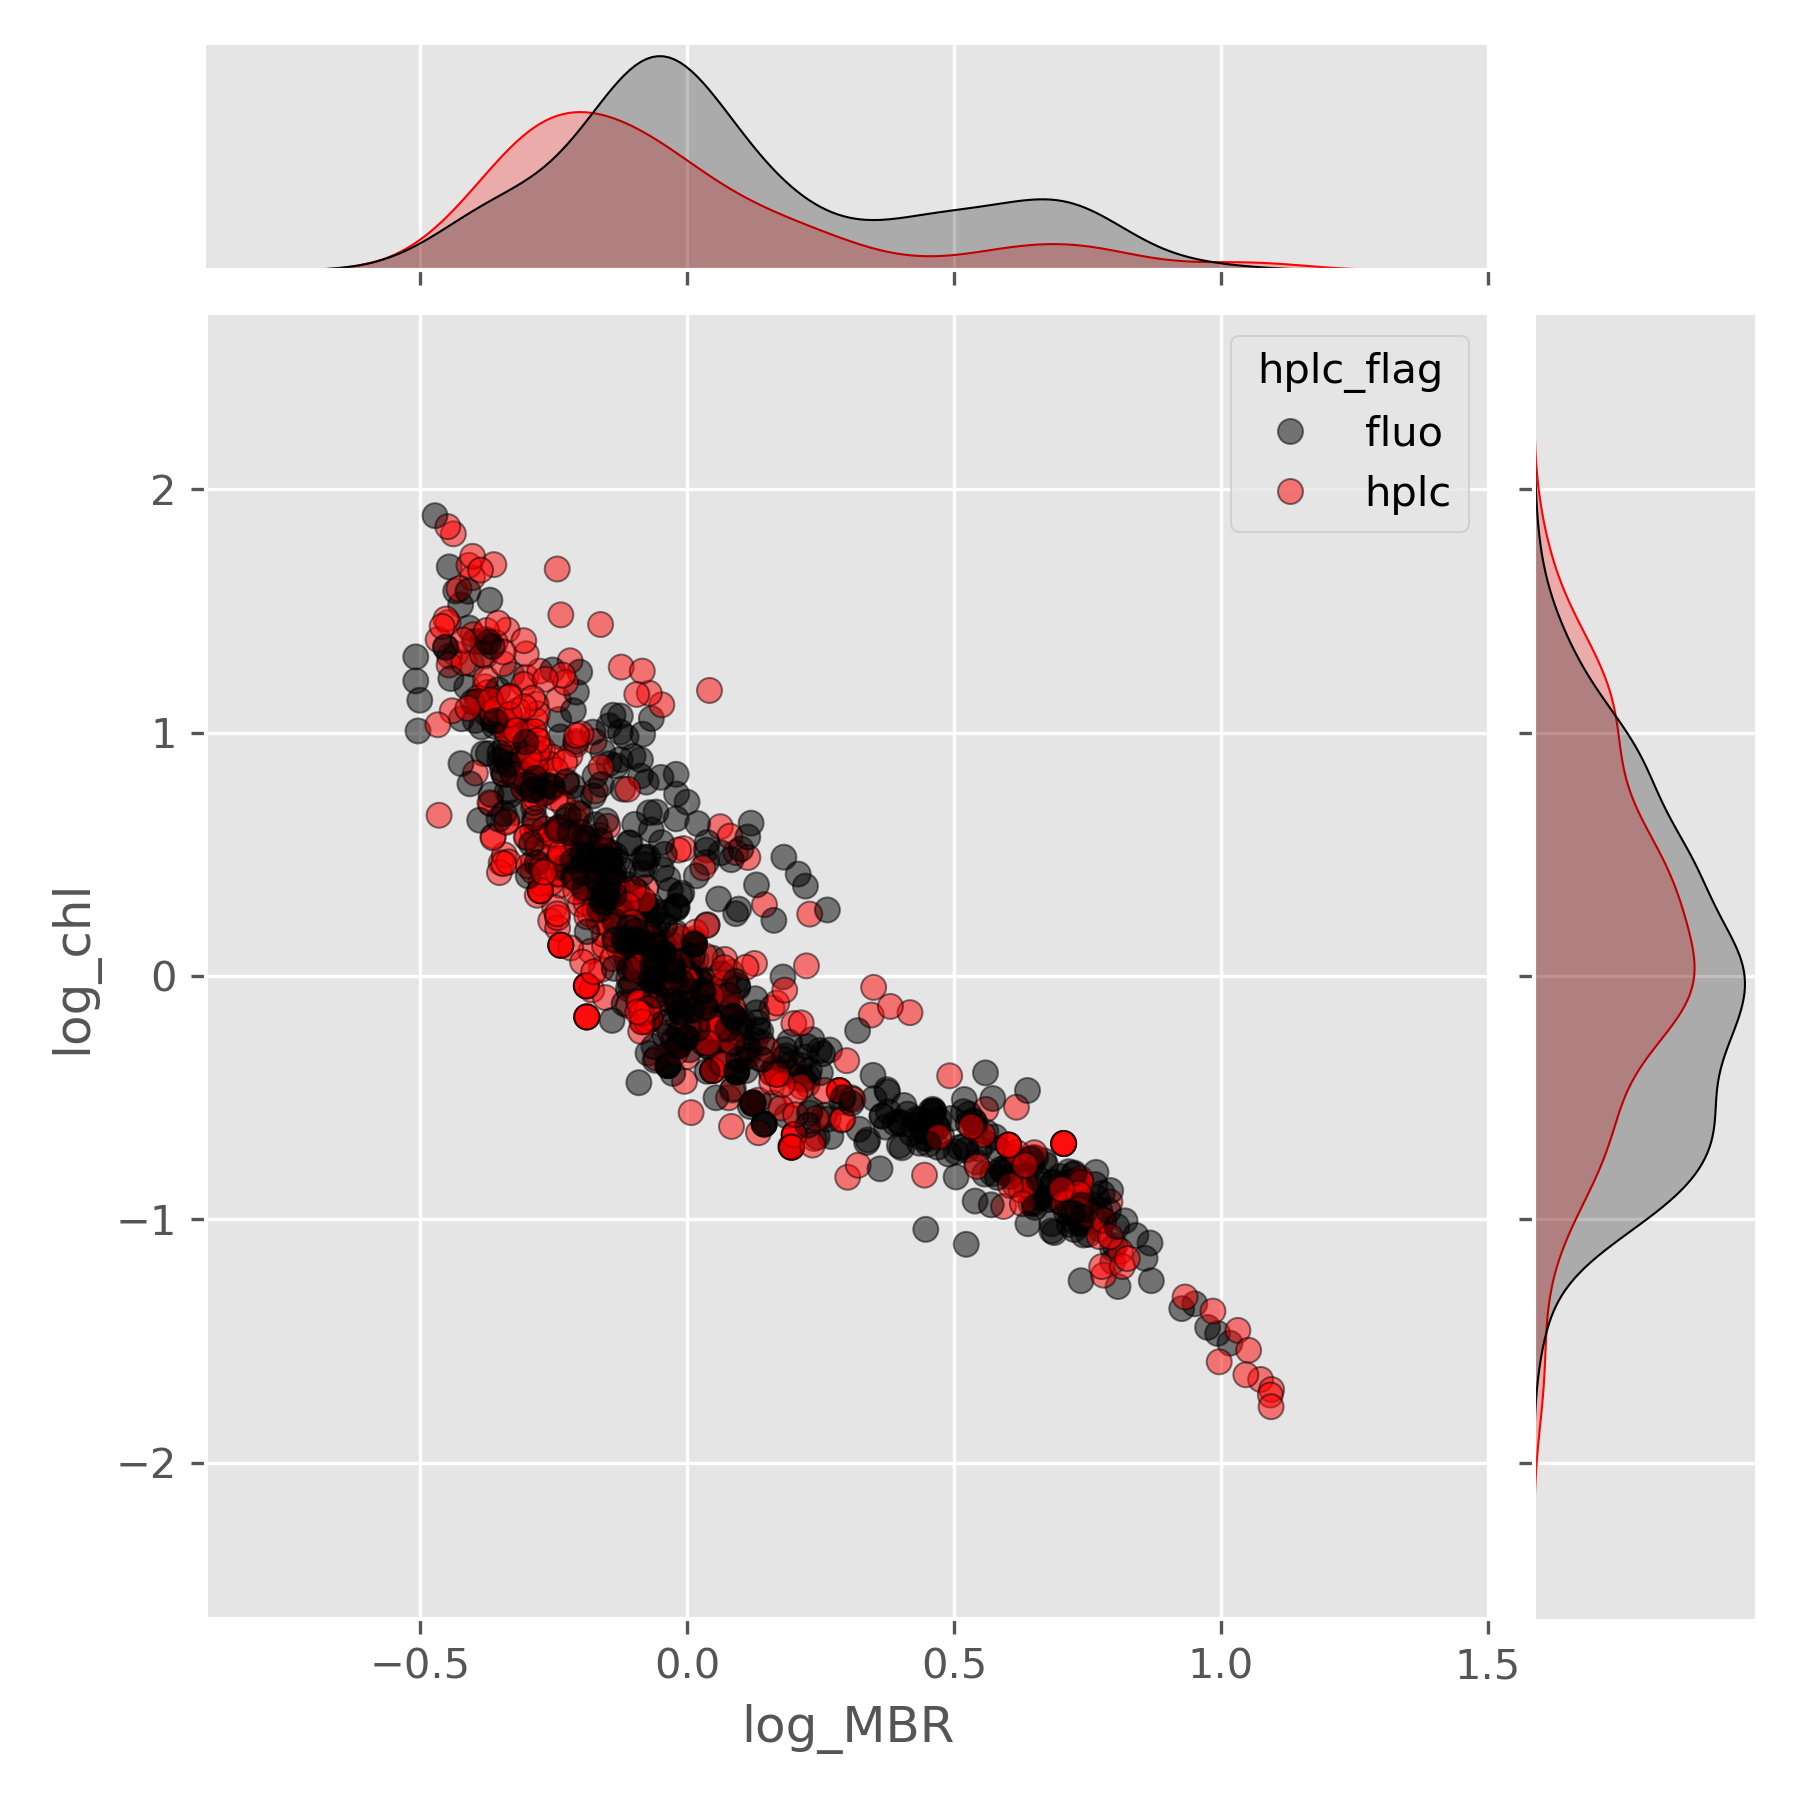
\includegraphics[keepaspectratio]{images/eda_hplc.png}}

}

\subcaption{\label{fig-eda-hplc}}

\end{minipage}%

\caption{\label{fig-eda}Two ways of grouping the data.
Figure~\ref{fig-eda-mbr}, max band ratio numerator;
Figure~\ref{fig-eda-hplc}, chlorophyll measurement method.}

\end{figure}%

\subsection{Bayesian Modeling
Framework}\label{bayesian-modeling-framework}

Several models of increasing levels were built. All models use
\(log(MBR)\) as primary input and \(log(chl)\) as target, some use
\(MBR\_flag\) as additional input, the last model also uses
\(hlpc_flag\). The following are key components shared across models.

\emph{Likelihood} - A truncated gaussian distribution with support
constrained to -3.0 to 3.2 on the \(log_{10}\) scale,corresponding to
\(0.001 - 1600 mg\ m^{-3}\) to reflect both detectable realistic levels
of marine surface chlorophyll.

\emph{Noise Structure} - Noise was incorporated as likelihood dispersion
parameter \(σ\); some of the models use a constant \(σ\), others take
heteroscedasticity into account.

\emph{Priors} - To estimate model posterior distribution, and produce
predictions with uncertainty following data fitting, all model
parameters receive a prior distribution, making explicit model
assumptions. Often there will be enough data to overrule the priors,
which are here mostly a conduit to the Posterior. An important caveat is
that care should be taken not to assign a 0-probability through a poorly
specified prior where support might actually be needed. Less
importantly, more efficient use of the search space can be done through
priors that assign 0-probability where support is clearly unreasonable.
Thus, all regression parameters receive Normal (Gaussian) 0-centered
weakly informative priors. And all \(σ\) terms received Gamma priors
that provide flexible but strictly positive support.

\emph{Software} - All models were implemented with the Python
probabilistic programming library PyMC V.5 (Abril-Pla et al., 2023) and
estimated using a variant of Hamiltonian Monte Carlo known as the
No-U-Turn Sampler (NUTS). Model diagnostics inference evaluation and
model comparisons were done through the Arviz package.

\subsection{Overview of Candidate
Models}\label{overview-of-candidate-models}

I developed six models representing a progression of modeling complexity
and assumptions:

\begin{itemize}
\tightlist
\item
  \textbf{Model 1}: Polynomial regression (Bayesian OC6-style
  baseline)\\
\item
  \textbf{Model 2}: Hierarchical linear regression, grouped by dominant
  MBR numerator band\\
\item
  \textbf{Model 3}: Similart to Model 2, with group-specific constant
  likelihood variance\\
\item
  \textbf{Model 4}: Global linear heteroscedastic model\\
\item
  \textbf{Model 5}: Similar to Model 2, with group-wise linear
  heteroscedasticity\\
\item
  \textbf{Model 6}: Model 6 plus an added dispersion term for
  fluorescence-based measurements
\end{itemize}

The main text focuses on Models 1, 2, 5, and 6, which span the range of
key structural variations. Full equations, priors, and diagnostic
results for all models are provided in the Supplement.

\subsection{Representative Model
Structures}\label{representative-model-structures}

Models are described here as sets of equations and Directed Acyclic
Graphs (DAG), with the former providing numerical details while the
latters helps visualize model structure and flow.

\subsubsection{Model 1: Bayesian 4th Order Polynomia
Regression}\label{model-1-bayesian-4th-order-polynomia-regression}

This model follows the OC6 formulation proposed by O'Reilly et
al.~(2019), with the difference that the denominator is the sum of
\(Rrs555\) and \(Rrs670\) rather than the mean. The model mean is a
fourth-order polynomial of \(log(MBR)\) to estimate \(log(Chl)\). The
set of proabilistic equations that define this model can be found in the
Supplemental Material Section. The model structure and inference flow is
represented in Figure~\ref{fig-model1-struct} as a Directed Acyclic
Graph (DAG).

\begin{figure}

\centering{

\pandocbounded{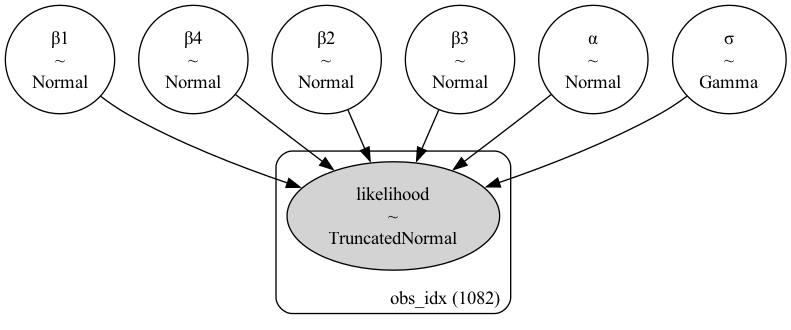
\includegraphics[keepaspectratio]{images/model1_structure.png}}

}

\caption{\label{fig-model1-struct}Model 1 Directed Acyclic Graph showing
model parameters and their prior distributions and how they relate . The
intercept \(α\) and the polynomial slopes, \(β1\)-\(β4\) all have
Gaussian priors; \(σ\), the likelihood dispersion parameter, receives a
Gamma prior; the likelihood itself is constrained by a Truncated Normal
distribution (see text for more). The plate containing the likelihood is
indexed (\(obs\_idx\)) indicating the likelihood will be computed for
each of the 1082 observations available.}

\end{figure}%

\subsubsection{Model 2: Hierarchical Linear Regression
(HLR)}\label{model-2-hierarchical-linear-regression-hlr}

\emph{Model 2} introduces partial pooling across four groups defined by
the dominant MBR numerator band; Rrs411, Rrs443, Rrs489, Rrs510
(\emph{cf}. Figure~\ref{fig-eda-mbr}). Each group receives its own slope
and intercept, and these parameters have shared hyperpriors.
Consequently, each group has its own sub-model that can capture details
specific to it and the shared hyperpriors allow for the sharing of
information between groups when fitting the model. This approach
maximizes the use of information contained in the available data.
Hierarchical models are usually result in uncertainty shrinkage.
Mathematical description of the model can be found in the Supplementary
Material. Figure~\ref{fig-model2-struct} illustrates the model
structure.

\begin{figure}

\centering{

\pandocbounded{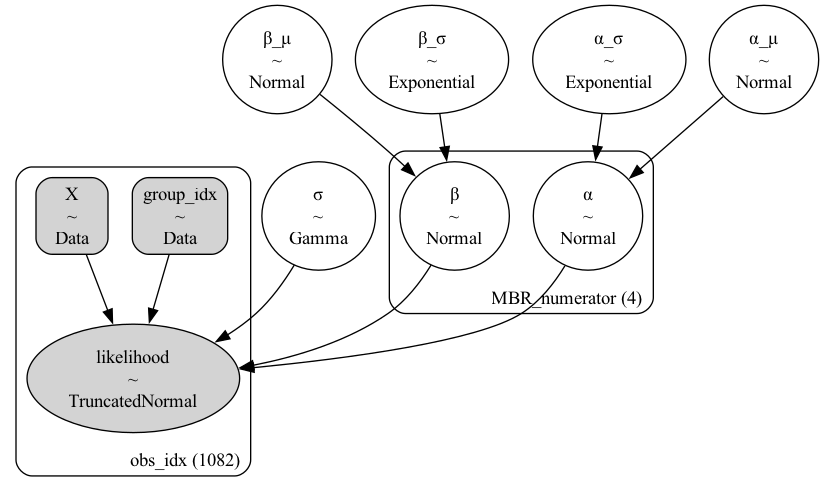
\includegraphics[keepaspectratio]{images/model2_structure.png}}

}

\caption{\label{fig-model2-struct}}

\end{figure}%

\subsubsection{Model 5: HLR with Added Linear Heteroscedastic Likelihood
Dispersion}\label{model-5-hlr-with-added-linear-heteroscedastic-likelihood-dispersion}

The data plotted in Figure~\ref{fig-eda} suggests heteroscedasticity -
variance that is not constant, but rather changes depending on the data.
Models 3 and 4 investigate the role of group-wise constant
heteroscedasticity and global linear heteroscedasticity, respectively.
Details of these models can be found in the Supplementary Material
section. To investigate this further, Model 5 looks at group-wise linear
heteroscedasticity. Thus, for a given MBR group \(j\) \(σ_j\) is modeled
as a log-linear relationship such that \(log(σ) = α_j + β_j × log(MBR)\)
and then transformed via \(exp(log(σ_j))\) before being passed on to the
likelihood. Similar to the model mean, \(μ_j\), \(σ_j\)'s slope and
intercept terms are partially pooled and so have common hyperpriors.
Mathematical descriiption of the model can be found in the Supplementary
Material section; Figure~\ref{fig-model5-struct}. illustrates the model
structure.

\begin{figure}

\centering{

\pandocbounded{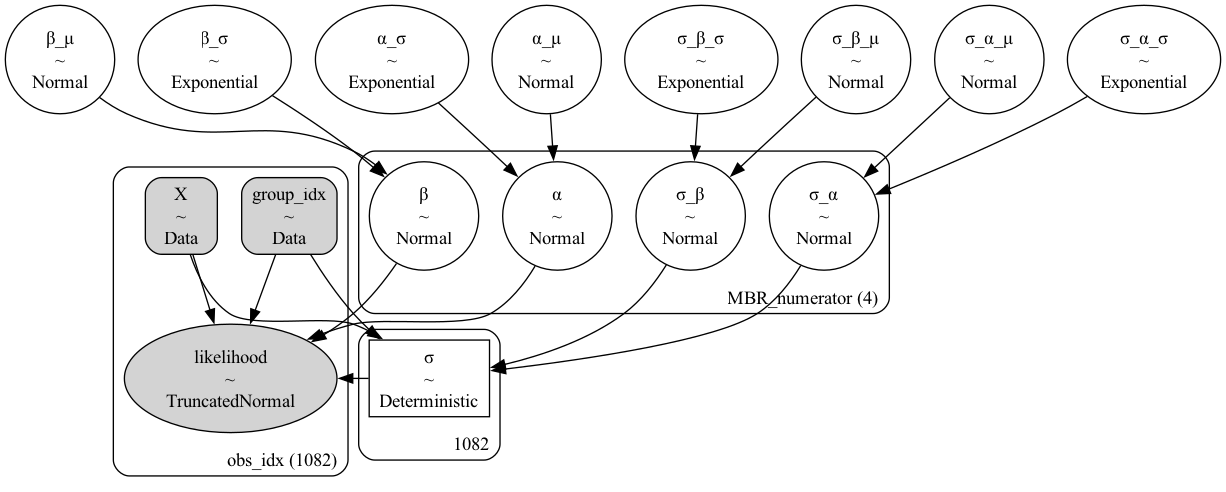
\includegraphics[keepaspectratio]{images/model5_structure.png}}

}

\caption{\label{fig-model5-struct}}

\end{figure}%

\subsubsection{Model 6: Augmenting Model 5 with Measurement-Specific
Dispersion}\label{model-6-augmenting-model-5-with-measurement-specific-dispersion}

A reasonable assumption is that HPLC measurements are less noisy than
fluorescence. This model adds a measurement-method-specific dispersion
term to the structure of Model 6, to capture the suspected increase in
variability associated with fluorescence-based chlorophyll estimates.
The likelihood dispersion, \(σ\), is given the expression
\(log(σ) = α_j + β_j × log(MBR) + γ_{chl\_type} * (1 - chl_{type\_idx})\),
where \(chl_{type\_idx} = 1\) if \emph{in-situ} chlorophyll was measured
with HPLC, \(0\) otherwise. As a result, \(σ\) is the same as in Model 5
if \(chl_{type\_idx} = 1\), since the extra term is nullified. In the
case of fluorescence measurement, on the other hand, \(log(σ)\) receives
an extra noise term, providing an effective measurement of noise
difference between the two methods. Figure~\ref{fig-model6-struct} shows
the inference DAG of Model 6.

\begin{figure}

\centering{

\pandocbounded{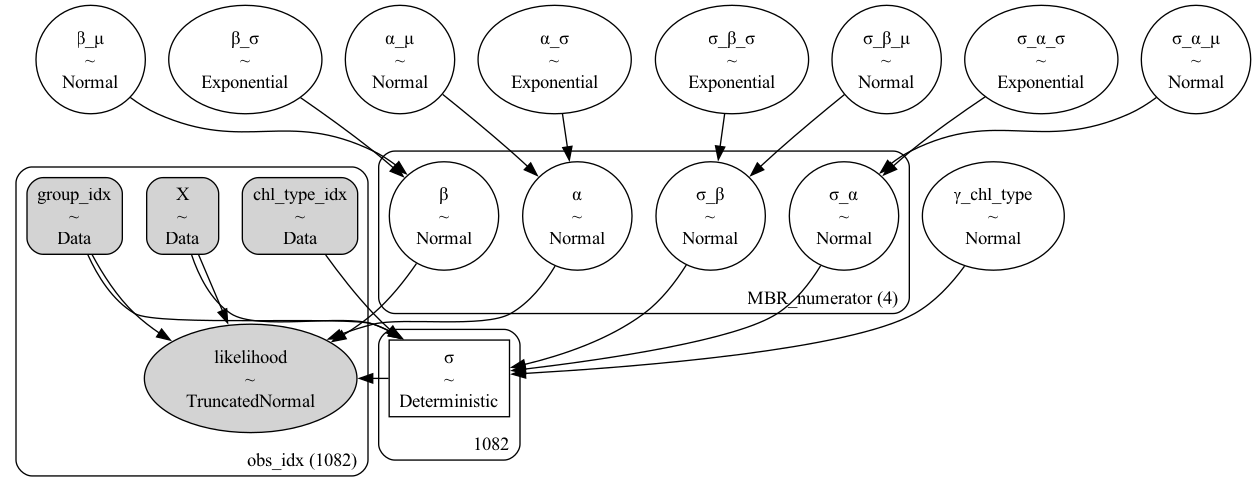
\includegraphics[keepaspectratio]{images/model6_structure.png}}

}

\caption{\label{fig-model6-struct}Model 6 - Similar to Model 5;
multi-level hierarchical linear model partial pooling across \(MBR\)
groups (Rrs411, Rrs443, Rrs489, Rrs510) for both model mean and
variance. However the linear variance model gets an additional parameter
\(γ\) that allows for the model dispersion to depend on the chlorophyll
measurement method (fluorescence or HPLC). While this does not
necessarily affect future , for which ground truth mearuement are
optional, it does allow the development of insight on the effect of
chloroophyll measurement method on model ucertainty.}

\end{figure}%

\subsection{Prior Specifications and Model
Fitting}\label{prior-specifications-and-model-fitting}

\emph{Priors} - I used weakly informative priors across all models to
balance flexibility with regularization. For regression parameters I
used Gaussian priors, In the case of the single-level Model 1, this
meant priors with \(0\) mean and variance of \(1\) to encourage
parameter sparsity. In the case of Models 2-6, which are multi-level
models, hyperpriors of prior means were set to Gaussans of mean 0 and
variance 1, again to encourage sparsity. Variance hyperpriors were given
Exponential distributions with rate set to \(1\) with significant
density near 0, whichß encourages similarity across groups unless the
data mandates otherwise. This hyperprior also encourages uncertainty
shrinkage across groups if possible. In the case of homoscedasticity, or
group-wise heteroscedasticity, I used a Gamma prior of shape and scale
of \(2\) for the likelihood dispersion \(σ\), which provides strictly
postivie support. Prior soundness was assessed using \emph{Prior
Predictive Checks}. This procedure takes advantage of the fact taht
Bayesian models are generative, meaning the model can be sampled without
data, to insure that values of (\(log(Chl)\)) predicted by the model are
reasonable even before model fitting. Prior predictive \(log(Chl)\)
values were plotted as Cumulative Distribution Function (CDF) of
\(log(Chl)\). Figure~\ref{fig-model1-priorpc} shows such a plot for
Model 1.

\begin{figure}

\centering{

\pandocbounded{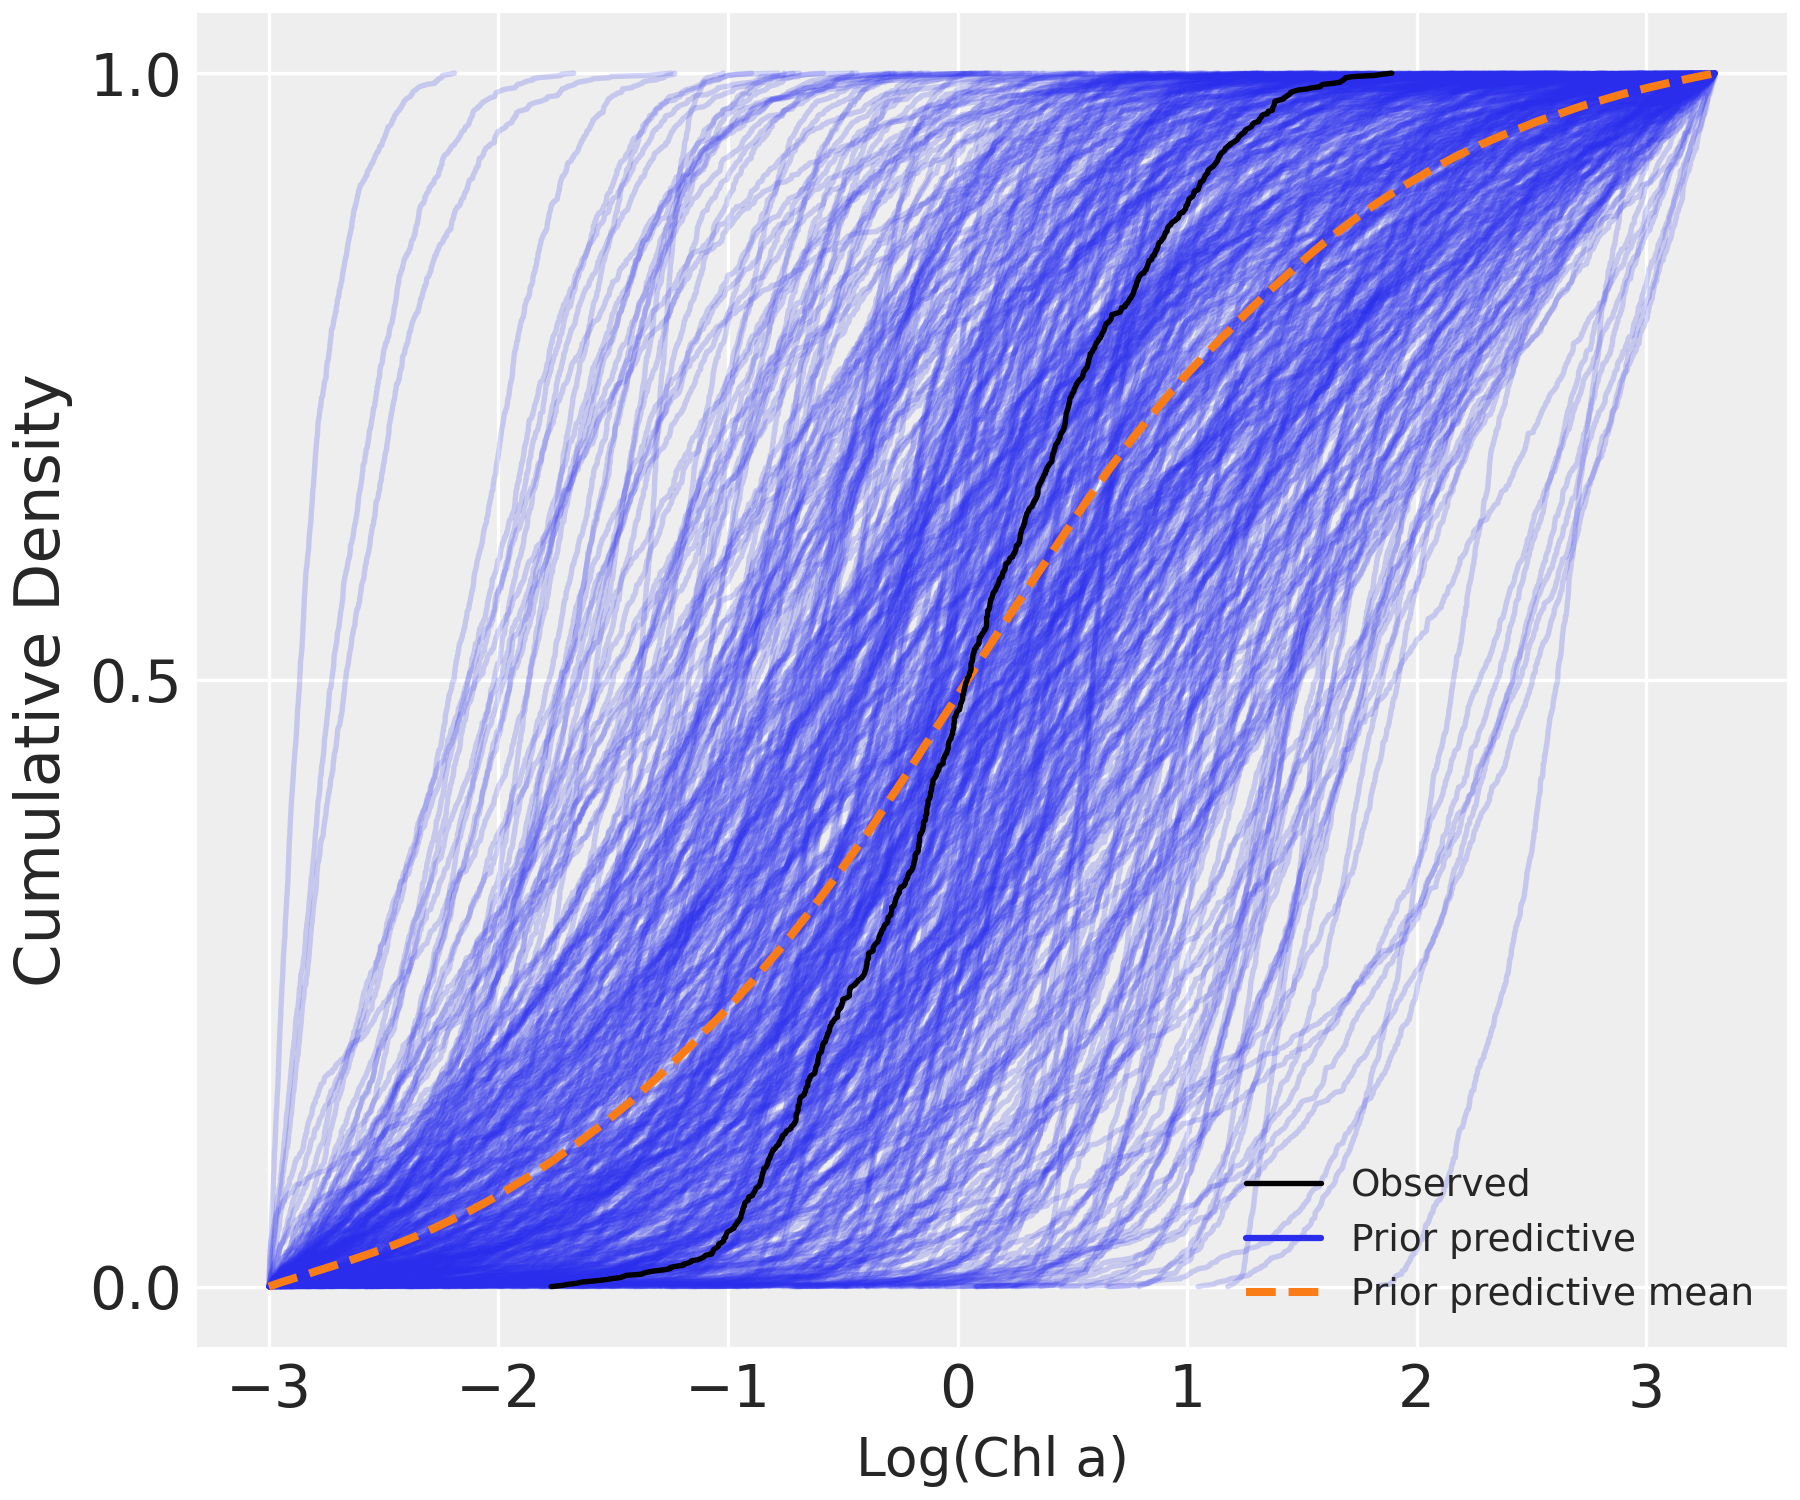
\includegraphics[keepaspectratio]{images/model1_prior.png}}

}

\caption{\label{fig-model1-priorpc}Prior Predictive Checks, here shown
for Model 1. This step allows the practitioner to verify the soundness
of model assumptions - choice of priors, the model formulation, etc.
This can be done even before data is collected as the generative nature
of Bayesian models means output can be produce based solely on the
priors and the model's mathematical expression alone. Results are
presented as Cumulative Distribution Function. In blue, 500 draws were
performed each containing a prescribed number of observations. The
dashed line represents the CDF of the simulation mean, In black, the CDF
of the data is shown for comparison.}

\end{figure}%

See \emph{Results} section for a Prior Predictive Checks plot example;
plots for all models can be found in the Supplementary Material section.

\emph{Model Fitting} - The model posterior was approximated using the No
U-Turn Sampler (NUTS), an efficient and mature variant of Hamiltonian
Monte Carlo (HMC), which uses particle physics to sample the posterior;
see the Supplementary Materials section for more details. Sampler
settings were as follows. Four independent sampling runs referred to as
\emph{chains} were used to assess sampler convergence. Prior to
sampling, 1000 tuning steps were used for each chain to maximize sampler
efficiency. The 2000 samples were recorded for each chain totalling 8000
samples. I assessed sampler convergence using the Gelman-Rubin
statistic, \(\hat{R}\) and effective sample size(\(ESS\)). Convergence
is acceptable for \(\hat{R}\) \textless{} 1.01 and \(ESS > 1000\). Full
trace plots and diagnostics are included in the Supplementary Material
section. Goodness of fit was assessed using \emph{Posterior plots},
which show *Posterior Predictive Checks, which show the expected

\subsection{Model Comparison and Predictive
Evaluation}\label{model-comparison-and-predictive-evaluation}

I compared model performance using \textbf{Pareto Smoothed Importance
Sampling Leave-One-Out Cross-Validation (PSIS-LOO-CV)} (Vehtari et al.,
2017). This Bayesian metric estimates the expected log predictive
density (ELPD), a principled measure of out-of-sample predictive
accuracy, that uses the entire posterior predictive distribution

\begin{itemize}
\tightlist
\item
  Models were ranked by ELPD\\
\item
  ΔELPD values were interpreted relative to their standard errors\\
\item
  Pareto-k diagnostics confirmed LOO reliability (full table in
  Supplement)
\end{itemize}

I evaluated predictive accuracy and calibration using:

\begin{itemize}
\tightlist
\item
  \textbf{Posterior Predictive Checks (PPCs)}:

  \begin{itemize}
  \tightlist
  \item
    Simulated draws overlaid on observed distributions\\
  \item
    Empirical CDF comparisons and interval coverage
  \end{itemize}
\item
  \textbf{HDI coverage}:

  \begin{itemize}
  \tightlist
  \item
    Fraction of observed values falling within 95\% posterior predictive
    intervals
  \end{itemize}
\end{itemize}

No frequentist evaluation criteria such as RMSE, MAE, or R² were used at
any stage as these do not make sense in this context where for each
observations, a probability distribution of the prediction is produced.

\section{Results}\label{results}

This section presents the outputs of posterior inference, model
comparison using Bayesian criteria, and posterior predictive diagnostics
for the four primary models. Results from the three supplementary models
are provided separately in the Supplement.

\subsection{MCMC Convergence}\label{mcmc-convergence}

All four models converged successfully. The Gelman-Rubin statistic
(R-hat ≈ 1.0) and large effective sample sizes (ESS \textgreater{} 1000)
across all parameters indicate robust posterior estimation. Diagnostic
plots and sampling traces are provided in the Supplementary Material.

\begin{itemize}
\tightlist
\item
  All R-hat \textless{} 1.01
\item
  No divergences
\item
  Sufficient tail and bulk ESS
\item
  Full diagnostics in Supplement
\end{itemize}

\subsection{Predictive Performance via Leave-One-Out Cross
Validation}\label{predictive-performance-via-leave-one-out-cross-validation}

We compared models using Pareto Smoothed Importance Sampling
Leave-One-Out Cross-Validation (PSIS-LOO-CV), a fully Bayesian approach
to evaluating out-of-sample predictive accuracy.

\textbf{Table 1.} Leave-One-Out Comparison (ELPD ± SE):

\begin{itemize}
\tightlist
\item
  Model 7 ranked highest in expected log predictive density (ELPD)
\item
  Model 6 performed comparably, with ΔELPD within 1 SE
\item
  Model 1 (OC6 polynomial) had the weakest predictive performance
\item
  All models had acceptable Pareto-k diagnostics (see Supplement)
\end{itemize}

\subsection{3.3 Posterior Predictive Checks
(PPC)}\label{posterior-predictive-checks-ppc}

We used posterior predictive checks (PPCs) to evaluate the ability of
each model to reproduce key features of the observed log-chlorophyll
distribution. These include:

\begin{itemize}
\tightlist
\item
  Empirical CDF comparisons
\item
  HDI envelopes overlaid on the data
\item
  Predictive median vs.~observed values
\end{itemize}

\textbf{Figure 1.} Posterior predictive envelopes vs.~observed
log(Chl)\\
\textbf{Figure 2.} ECDF overlays with posterior predictive means and
HDIs\\
\textbf{Figure 3.} Rug plot of observations with overlaid posterior
predictive draws

Findings: - Model 7 captures full data distribution, especially for
fluorescence-labeled values - Model 1 underestimates tails
(under-dispersed) - Model 6 accurately reflects group-level variance

\subsection{3.4 Posterior Distributions and
Interpretability}\label{posterior-distributions-and-interpretability}

Posterior distributions for key parameters illustrate how model
structure affects inference. We show both: - Group-level slopes and
intercepts (hierarchical structure) - Group-wise σ (heteroscedasticity)
- Fluorescence-specific variance term (Model 7)

\textbf{Figure 4.} Forest plot of slope and intercept posteriors\\
\textbf{Figure 5.} Posterior of σ across MBR groups\\
\textbf{Figure 6.} Posterior of added noise term for fluorescence

Key insights: - Rrs510-dominant group had the steepest slope (Model 2 \&
6) - Fluorescence noise term is credibly nonzero (Model 7) - Posterior
variance structure supports heteroscedasticity as a key feature

\subsection{3.5 Summary of Bayesian
Comparison}\label{summary-of-bayesian-comparison}

\begin{itemize}
\tightlist
\item
  \textbf{Model 7}: Best predictive performance (highest ELPD), best
  uncertainty calibration
\item
  \textbf{Model 6}: Nearly equivalent performance; simpler if
  fluorescence uncertainty not needed
\item
  \textbf{Model 2}: Gains from partial pooling; underperforms without
  variance modeling
\item
  \textbf{Model 1}: Legacy structure underfits tails, overconfident
  predictions
\end{itemize}

All results support the Bayesian hierarchical modeling framework with
heteroscedasticity and measurement-aware noise as optimal for
chlorophyll-a estimation.

\section{4. Discussion}\label{discussion}

This section interprets the results in the context of previous
chlorophyll-a modeling work, with particular emphasis on the added value
of Bayesian modeling. We highlight the importance of accounting for
heteroscedasticity and measurement-type uncertainty, and discuss how
this contributes to improved predictive reliability and scientific
interpretability.

\subsection{4.1 Value of Bayesian Framework over Classical
Approaches}\label{value-of-bayesian-framework-over-classical-approaches}

Our results demonstrate the clear advantages of fully Bayesian modeling
for chlorophyll-a prediction from satellite Rrs. Unlike deterministic or
frequentist models:

\begin{itemize}
\tightlist
\item
  Bayesian methods explicitly model parameter uncertainty and provide
  HDIs instead of misleading confidence intervals
\item
  Posterior predictive distributions enable direct evaluation of model
  calibration
\item
  Bayesian model comparison via LOO-CV avoids overfitting and guards
  against inappropriate complexity
\end{itemize}

\subsection{4.2 Importance of Hierarchical
Structuring}\label{importance-of-hierarchical-structuring}

Models that leveraged group-wise structure (based on dominant Rrs bands)
consistently outperformed simpler counterparts.

\begin{itemize}
\tightlist
\item
  Hierarchical partial pooling improved both prediction and parameter
  identifiability
\item
  Group-level trends reflected known biogeophysical distinctions (e.g.,
  clear vs.~turbid water types)
\item
  Intercepts and slopes varied systematically across spectral regimes
\end{itemize}

\subsection{4.3 Role of Heteroscedasticity in Chlorophyll
Retrieval}\label{role-of-heteroscedasticity-in-chlorophyll-retrieval}

Accounting for non-constant noise was essential for accurate uncertainty
quantification.

\begin{itemize}
\tightlist
\item
  Models with linear or hierarchical σ terms captured increased variance
  at higher MBR or Chl
\item
  Constant-σ models (e.g., OC6) underrepresented predictive uncertainty,
  especially in extremes
\item
  Explicit modeling of σ structure produced calibrated HDIs and superior
  posterior predictive checks
\end{itemize}

\subsection{4.4 Measurement-Specific Error
Modeling}\label{measurement-specific-error-modeling}

Model 7, which introduced a separate noise term for fluorescence-derived
Chl, outperformed all others.

\begin{itemize}
\tightlist
\item
  Fluorescence-based measurements have higher and more variable error
\item
  This heterogeneity cannot be ignored in merged datasets
\item
  Bayesian modeling allows this variance to be encoded explicitly
  without discarding data
\end{itemize}

\subsection{4.5 Implications for Satellite Algorithm
Development}\label{implications-for-satellite-algorithm-development}

The findings support incorporating Bayesian elements into future
operational chlorophyll algorithms.

\begin{itemize}
\tightlist
\item
  Hierarchical modeling offers a path to generalize across bioregions
  and sensors
\item
  Posterior uncertainty estimates can support downstream applications
  (e.g., forecasting, ecological thresholds)
\item
  Bayesian frameworks are sensor-agnostic: Rrs inputs can vary as long
  as priors are adapted
\end{itemize}

\subsection{4.6 Limitations and Future
Work}\label{limitations-and-future-work}

As with any modeling effort, our study has limitations:

\begin{itemize}
\tightlist
\item
  All results are conditional on the data from NOMAD; further validation
  on independent datasets is needed
\item
  More sophisticated noise structures (e.g., nonparametric σ) could be
  explored
\item
  Spatial or spatio-temporal extensions were not considered, but would
  be feasible in PyMC
\end{itemize}

\section{Acknowledgments}\label{acknowledgments}

\section{Open research}\label{open-research}

\section*{References}\label{references}
\addcontentsline{toc}{section}{References}

\phantomsection\label{refs}
\begin{CSLReferences}{1}{0}
\vspace{1em}

\bibitem[\citeproctext]{ref-abril2023pymc}
Abril-Pla, O., Andreani, V., Carroll, C., Dong, L., Fonnesbeck, C. J.,
Kochurov, M., et al. (2023). PyMC: A modern, and comprehensive
probabilistic programming framework in python. \emph{PeerJ Computer
Science}, \emph{9}, e1516. \url{https://doi.org/10.7717/peerj-cs.1516}

\bibitem[\citeproctext]{ref-baker2016}
Baker, M. (2016). 1,500 scientists lift the lid on reproducibility.
\emph{Nature}, \emph{533}(7604), 452--454.
\url{https://doi.org/10.1038/533452a}

\bibitem[\citeproctext]{ref-bishop2006pattern}
Bishop, C. M. (2006). \emph{Pattern recognition and machine learning}.
Springer.

\bibitem[\citeproctext]{ref-clayton2022bernoulli}
Clayton, A. (2022). \emph{Bernoulli's fallacy: Statistical illogic and
the crisis of modern science}. Columbia University Press. Retrieved from
\url{https://books.google.com/books?id=BT4CzwEACAAJ}

\bibitem[\citeproctext]{ref-cobey2024biomedical}
Cobey, K. D., Ebrahimzadeh, S., Page, M. J., Thibault, R. T., Nguyen,
P.-Y., Abu-Dalfa, F., \& Moher, D. (2024). Biomedical researchers'
perspectives on the reproducibility of research. \emph{PLoS Biology},
\emph{22}(11), e3002870.

\bibitem[\citeproctext]{ref-craig2019}
Craig, S. E., \& Karaköylü, E. M. (2019). Bayesian models for deriving
biogeochemical information from satellite ocean color.
\emph{EarthArXiv}. \url{https://doi.org/10.31223/osf.io/shp6y}

\bibitem[\citeproctext]{ref-erickson2023}
Erickson, Z. K., McKinna, L. I. W., Werdell, P. J., \& Cetinić, I.
(2023). Bayesian approach to a generalized inherent optical property
model. \emph{Optics Express}, \emph{31}, 22790--22801.
\url{https://doi.org/10.1364/oe.486581}

\bibitem[\citeproctext]{ref-frouin2013}
Frouin, R., \& Pelletier, B. (2013). Bayesian methodology for ocean
color remote sensing. Retrieved from
\url{https://hal.archives-ouvertes.fr/hal-00822032}

\bibitem[\citeproctext]{ref-gal2016uncertainty}
Gal, Y. (2016). \emph{Uncertainty in deep learning} (PhD thesis).
University of Cambridge.

\bibitem[\citeproctext]{ref-hu2012novel}
Hu, C., Lee, Z., \& Franz, B. (2012). Chlorophyll aalgorithms for
oligotrophic oceans: A novel approach based on three-band reflectance
difference. \emph{Journal of Geophysical Research: Oceans},
\emph{117}(C1).
https://doi.org/\url{https://doi.org/10.1029/2011JC007395}

\bibitem[\citeproctext]{ref-hu2019improving}
Hu, C., Feng, L., Lee, Z., Franz, B. A., Bailey, S. W., Werdell, P. J.,
\& Proctor, C. W. (2019). Improving satellite global chlorophyll a data
products through algorithm refinement and data recovery. \emph{Journal
of Geophysical Research: Oceans}, \emph{124}(3), 1524--1543.
https://doi.org/\url{https://doi.org/10.1029/2019JC014941}

\bibitem[\citeproctext]{ref-jaynes2003probability}
Jaynes, E. T., \& Bretthorst, G. L. (2003). \emph{Probability theory:
The logic of science}. Cambridge University Press. Retrieved from
\url{https://books.google.com/books?id=tTN4HuUNXjgC}

\bibitem[\citeproctext]{ref-oreilly2019}
O'Reilly, John E., \& Werdell, P. J. (2019). Chlorophyll algorithms for
ocean color sensors - OC4, OC5 \& OC6. \emph{Remote Sensing of
Environment}, \emph{229}, 32--47.
https://doi.org/\url{https://doi.org/10.1016/j.rse.2019.04.021}

\bibitem[\citeproctext]{ref-oreilly1998}
O'Reilly, John E., Maritorena, S., Mitchell, B. G., Siegel, D. A.,
Carder, K. L., Garver, S. A., et al. (1998). Ocean color chlorophyll
algorithms for SeaWiFS. \emph{Journal of Geophysical Research: Oceans},
\emph{103}(C11), 24937--24953.
https://doi.org/\url{https://doi.org/10.1029/98JC02160}

\bibitem[\citeproctext]{ref-oreilly2000}
O'Reilly, John E., Maritorena, S., Siegel, D. A., O'Brien, M. C., Toole,
D., Mitchell, B. G., et al. (2000). Ocean color chlorophyll a algorithms
for SeaWiFS, OC2, and OC4: Version 4. \emph{SeaWiFS Postlaunch
Calibration and Validation Analyses, Part}, \emph{3}, 9--23.

\bibitem[\citeproctext]{ref-seegers2018}
Seegers, B. N., Stumpf, R. P., Schaeffer, B. A., Loftin, K. A., \&
Werdell, P. J. (2018). Performance metrics for the assessment of
satellite data products: An ocean color case study. \emph{Opt. Express},
\emph{26}(6), 7404--7422. \url{https://doi.org/10.1364/OE.26.007404}

\bibitem[\citeproctext]{ref-reback2020pandas}
team, T. pandas development. (2020, February). Pandas-dev/pandas: pandas
(Version latest). Zenodo. \url{https://doi.org/10.5281/zenodo.3509134}

\bibitem[\citeproctext]{ref-vehtari2017}
Vehtari, A., Gelman, A., \& Gabry, J. (2017). Practical bayesian model
evaluation using leave-one-out cross-validation and WAIC.
\emph{Statistics and Computing}, \emph{27}(5), 1413--1432.
\url{https://doi.org/10.1007/s11222-016-9696-4}

\bibitem[\citeproctext]{ref-werdell2005improved}
Werdell, P. J., \& Bailey, S. W. (2005). An improved bio-optical data
set for ocean color algorithm development and satellite data product
validation. \emph{Remote Sensing of Environment}, \emph{98}(1),
122--140.

\end{CSLReferences}




\end{document}
